
\subsubsection[Hierarchical (AGNES e DIANA)]{Hierarchical \textit{(AGNES e DIANA)}}
\begin{frame}

	\frametitle{{\color{GradientDescentDiagramGreen}Hierarchical Clustering}, in sintesi}

	%\begin{block}{}
		Il clustering gerarchico crea un albero di clusters.\\
		È una metodologia di clustering che cerca di costruire una gerarchia di cluster, rappresentata con un albero che prende il nome di \emph{dendogramma}.\newlinedouble
		%Mira a creare una sorta di tassonomia al variare del numero di clusters $K$.\\ %  da $1$ a $N$ dove $N$ è il numero di osservazioni del dataset.
		È possibile decidere un numero $K$ qualsiasi di clusters per il nostro specifico problema tagliando l'albero costruito con tale procedura al giusto livello.
		\begin{figure}[!htbp]
			\centering
			\includegraphics[width=7.0cm]{images/unsupervised/types/Clustering_Hierarchical.pdf}
					%\caption{Stripe Radar for Fraud Detection}
		\end{figure}
	%\end{block}

\end{frame}


\begin{frame}

	\frametitle{{\color{GradientDescentDiagramGreen}Hierarchical Clustering}}

%	\begin{block}{Idea di base}
		Il clustering gerarchico può essere suddiviso in due tipologie principali:
		\begin{itemize}
			\item \textbf{clustering gerarchico agglomerativo}: è noto anche come \textbf{AGNES} (Agglomerative Nesting, bottom-up). Cioè, ogni oggetto viene inizialmente considerato come un cluster a elemento singolo (foglia). Ad ogni passaggio dell'algoritmo, i due cluster più simili vengono combinati in un nuovo cluster più grande (nodi). Questa procedura viene ripetuta finché tutti i punti non sono membri di un unico grande cluster (radice). Il risultato è un albero che può essere tracciato come un dendrogramma.
			\item \textbf{clustering gerarchico divisivo}: è noto anche come \textbf{DIANA} (Divise Analysis, top-down). L'algoritmo procede in ordine inverso rispetto all'AGNES. Inizia con la radice, in cui tutti gli oggetti sono inclusi in un singolo cluster. In ogni fase dell'iterazione, il cluster più eterogeneo viene diviso in due. Il processo viene iterato fino a quando tutti gli oggetti si trovano nel loro proprio cluster.
		\end{itemize}
%	\end{block}
\end{frame}


\begin{frame}

	\frametitle{{\color{GradientDescentDiagramGreen}Hierarchical Clustering}}

%	\begin{block}{Idea di base}
		\ifthenelse{\boolean{highschool}}{}{Si noti che il clustering agglomerativo è utile per identificare piccoli cluster. Il clustering divisivo è utile per identificare cluster di grandi dimensioni.}
		\begin{figure}[!htbp]
			\centering
			\includegraphics[width=12.0cm]{images/unsupervised/hierarchical/hierarchical-clustering-agnes-diana.png}
					%\caption{Stripe Radar for Fraud Detection}
		\end{figure}

%	\end{block}
\end{frame}



\begin{frame}

	\frametitle{{\color{GradientDescentDiagramGreen}Hierarchical Clustering}}

	\begin{block}{Clustering gerarchico agglomerativo: idea di base}
		\begin{itemize}
			\item agglomerare ricorsivamente i punti in cluster combinando i punti e i cluster più vicini per ottenere cluster più grandi fino a quando tutti i punti vengono raccolti in un solo cluster
		\end{itemize}
		Il processo ricorsivo definisce una gerarchia che rende esplicita la struttura del set di dati in termini di cluster di grandi dimensioni e sub-clusters.
		\newlinedouble
		Il clustering gerarchico richiede la specifica di come calcolare la distanza tra:
		\begin{itemize}
			\item due punti (Manhattan, Euclidean, cosine ...)
			\item un punto e un cluster (...)
			\item due cluster (...)
		\end{itemize}
	\end{block}

\end{frame}


\begin{frame}

	\frametitle{{\color{GradientDescentDiagramGreen}Hierarchical Clustering}}

	\begin{block}{Clustering gerarchico agglomerativo: algoritmo}
		\begin{enumerate}
			\item all'inizio, ogni punto definisce un nuovo cluster, risultando in N cluster ciascuno contenente un solo punto. Le distanze tra tutte le coppie di cluster vengono calcolate e memorizzate in una matrice $A_{NN}$
			\item trovare la coppia di cluster più vicina e unirli in un unico cluster. Calcola e memorizza la distanza tra il nuovo cluster e tutti gli altri (ovvero, aggiorna $A_{NN}$)
			\item ripeti il passaggio 2 fino a quando tutti i punti sono raggruppati in un unico cluster composto da $N$ punti
		\end{enumerate}
	\end{block}

\end{frame}


\begin{frame}

	\frametitle{{\color{GradientDescentDiagramGreen}Hierarchical Clustering}}

	\begin{block}{Metriche di dissimilarità più utilizzate: (indicate successivamente con $\bigstar$)}

		\begin{itemize}
			\item \textbf{Euclidean distance}:\\
				\makebox[\textwidth]{$d_{euc}(x,y) = \sqrt{\sum^n_{i=1}(x_i - y_i)^2}$}
			\item \textbf{Manhattan distance}:\\
				\makebox[\textwidth]{$d_{man}(x,y) = \sum^n_{i=1}|(x_i - y_i)|$}
			\item \textbf{Pearson correlation distance}:\\
				\makebox[\textwidth]{$d_{cor}(x, y) = 1 - \frac{\sum^n_{i=1}(x_i-\bar x)(y_i - \bar y)}{\sqrt{\sum^n_{i=1}(x_i-\bar x)^2\sum^n_{i=1}(y_i - \bar y)^2}}$}
			\ifthenelse{\boolean{highschool}}{
			\item \textbf{\underline{\href{https://uc-r.github.io/kmeans_clustering\#distance}{Altre...}}}}{
			\item \textbf{Spearman correlation distance}:\\
				\makebox[\textwidth]{$d_{spear}(x, y) = 1 - \frac{\sum^n_{i=1}(x^\prime_i-\bar x^\prime)(y^\prime_i - \bar y^\prime)}{\sqrt{\sum^n_{i=1}(x^\prime_i-\bar x^\prime)^2\sum^n_{i=1}(y^\prime_i - \bar y^\prime)^2}} \rightarrow$ \underline{\href{https://uc-r.github.io/kmeans_clustering\#distance}{link per dettagli}}}
			\item \textbf{Kendall correlation distance}:\\
				\makebox[\textwidth]{$d_{kend}(x,y) = 1 - \frac{n_c - n_d}{\frac{1}{2}n(n - 1)} \rightarrow$ \underline{\href{https://uc-r.github.io/kmeans_clustering\#distance}{link per dettagli}}}
			}
		\end{itemize}


	\end{block}

\end{frame}


\begin{frame}

	\frametitle{{\color{GradientDescentDiagramGreen}Hierarchical Clustering}}

	\begin{block}{La distanza tra due clusters $C_i$ e $C_j$ è calcolata come:}
		\begin{itemize}
			\item nel \textbf{single-link} clustering:\\
				come la \textit{minima distanza} tra un punto di $C_i$ e un punto di $C_j$\\
				\makebox[\textwidth]{$d_{SL}(C_i, C_j) = \underset{x \in C_i, y \in C_j}{min} d_{\bigstar}(x, y)$}
				\vspace{0.5mm}
			\item nel \textbf{average-link} clustering:\\
				come la \textit{distanza media} tra un punto di $C_i$ e un punto di $C_j$\\
				\makebox[\textwidth]{$d_{AVG}(C_i, C_j) = \underset{x \in C_i, y \in C_j}{avg} d_{\bigstar}(x, y)$}
				\vspace{0.5mm}
			\item nel \textbf{complete-link} clustering:\\
				come la \textit{massima distanza} tra un punto di $C_i$ e un punto di $C_j$\\
				\makebox[\textwidth]{$d_{CL}(C_i, C_j) = \underset{x \in C_i, y \in C_j}{max} d_{\bigstar}(x, y)$}
		\end{itemize}
		Esistono altre metriche di distanze tra clusters, vedi \underline{\href{https://uc-r.github.io/hc_clustering}{link per dettagli}}.
	\end{block}

\end{frame}


\begin{frame}

	\frametitle{{\color{GradientDescentDiagramGreen}Hierarchical Clustering}}

	%\begin{block}{}
		\begin{itemize}
			\item si noti che la distanza tra due cluster può essere misurata in modi diversi
			\item indipendentemente da ciò, ad ogni passaggio i due cluster più vicini vengono aggregati
			\item tipicamente, prima di iniziare il processo di clusterizzazione, i valori delle features vengono scalati in modo da avere media zero e deviazione standard unitaria
		\end{itemize}

	%\end{block}

\end{frame}


\begin{frame}

	\frametitle{{\color{GradientDescentDiagramGreen}Hierarchical Clustering}: Euclidean + Single-Link}

	%\begin{block}{}

		\begin{figure}[!htbp]
			\centering
			
			\includegraphics<1>[width=0.70\linewidth, height=7.2cm]{images/unsupervised/hierarchical/hierarchical_single_link_1.png}
			\includegraphics<2>[width=0.70\linewidth, height=7.2cm]{images/unsupervised/hierarchical/hierarchical_single_link_2.png}
			\includegraphics<3>[width=0.70\linewidth, height=7.2cm]{images/unsupervised/hierarchical/hierarchical_single_link_3.png}
			\includegraphics<4>[width=0.70\linewidth, height=7.2cm]{images/unsupervised/hierarchical/hierarchical_single_link_4.png}
			\includegraphics<5>[width=0.70\linewidth, height=7.2cm]{images/unsupervised/hierarchical/hierarchical_single_link_5.png}
			\includegraphics<6>[width=0.70\linewidth, height=7.2cm]{images/unsupervised/hierarchical/hierarchical_single_link_6.png}
			
			%\caption{Single-Link}
			%\label{Enel_HistFit_Normal}
		\end{figure}

	%\end{block}

\end{frame}


\begin{frame}

	\frametitle{{\color{GradientDescentDiagramGreen}Hierarchical Clustering}: Euclidean + Complete-Link}

	%\begin{block}{}

		\begin{figure}[!htbp]
			\centering
			
			\includegraphics<1>[width=0.70\linewidth, height=7.2cm]{images/unsupervised/hierarchical/hierarchical_complete_link_1.png}
			\includegraphics<2>[width=0.70\linewidth, height=7.2cm]{images/unsupervised/hierarchical/hierarchical_complete_link_2.png}
			\includegraphics<3>[width=0.70\linewidth, height=7.2cm]{images/unsupervised/hierarchical/hierarchical_complete_link_3.png}
			\includegraphics<4>[width=0.70\linewidth, height=7.2cm]{images/unsupervised/hierarchical/hierarchical_complete_link_4.png}
			\includegraphics<5>[width=0.70\linewidth, height=7.2cm]{images/unsupervised/hierarchical/hierarchical_complete_link_5.png}
			\includegraphics<6>[width=0.70\linewidth, height=7.2cm]{images/unsupervised/hierarchical/hierarchical_complete_link_6.png}
			
			%\caption{Complete-Link}
			%\label{Enel_QQ_Plot_Normal}
		\end{figure}

	%\end{block}

\end{frame}


\begin{frame}

	\frametitle{{\color{GradientDescentDiagramGreen}Hierarchical Clustering}}

	%\begin{block}{}

		\begin{columns}

			\column{0.5\linewidth}
			\begin{figure}[!htbp]
				\centering
				\includegraphics[angle=0,width=0.75\linewidth]{images/unsupervised/hierarchical/hierarchical_single_link.pdf}
				\caption{Euclidean + Single-Link}
				%\label{Enel_HistFit_Normal}
			\end{figure}

			\column{0.5\linewidth}
			\begin{figure}[!htbp]
				\centering
				\includegraphics[angle=0,width=0.75\linewidth]{images/unsupervised/hierarchical/hierarchical_complete_link.pdf}
				\caption{Euclidean + Complete-Link}
				%\label{Enel_QQ_Plot_Normal}
			\end{figure}

		\end{columns}

	%\end{block}

\end{frame}


\begin{frame}

	\frametitle{{\color{GradientDescentDiagramGreen}Hierarchical Clustering}}

	%\begin{block}{}

		La gerarchia dei cluster è rappresentata graficamente tramite un dendrogramma.\\
		Il dendogramma mostra a quali distanze i cluster sono raggruppati.

		\begin{columns}

			\column{0.5\linewidth}
			\begin{figure}[!htbp]
				\centering
				\includegraphics[angle=0,width=0.50\linewidth]{images/unsupervised/hierarchical/hierarchical_single_link.pdf}
				\caption{Single-Link}
				%\label{Enel_HistFit_Normal}
			\end{figure}

			\column{0.5\linewidth}
			\begin{figure}[!htbp]
				\centering
				\includegraphics[angle=0,width=0.65\linewidth]{images/unsupervised/hierarchical/hierarchical_single_link_dendogram.pdf}
				\caption{Single-Link Dendogram}
				%\label{Enel_QQ_Plot_Normal}
			\end{figure}

		\end{columns}

	%\end{block}

\end{frame}



\begin{frame}

	\frametitle{{\color{GradientDescentDiagramGreen}Hierarchical Clustering}}

	%\begin{block}{}

		La gerarchia dei cluster è rappresentata graficamente tramite un dendrogramma.\\
		Il dendogramma mostra a quali distanze i cluster sono raggruppati.

		\begin{columns}

			\column{0.5\linewidth}
			\begin{figure}[!htbp]
				\centering
				\includegraphics[angle=0,width=0.50\linewidth]{images/unsupervised/hierarchical/hierarchical_complete_link.pdf}
				\caption{Complete-Link}
				%\label{Enel_HistFit_Normal}
			\end{figure}

			\column{0.5\linewidth}
			\begin{figure}[!htbp]
				\centering
				\includegraphics[angle=0,width=0.65\linewidth]{images/unsupervised/hierarchical/hierarchical_complete_link_dendogram.pdf}
				\caption{Complete-Link Dendogram}
				%\label{Enel_QQ_Plot_Normal}
			\end{figure}

		\end{columns}

	%\end{block}

\end{frame}


\begin{frame}

	\frametitle{{\color{GradientDescentDiagramGreen}Hierarchical Clustering}}

	%\begin{block}{}

		I dendrogrammi possono aiutare a identificare un ``buon'' numero di cluster
		\begin{itemize}
			\item un ampio gap nelle distanze suggerisce quando interrompere il processo di raggruppamento
		\end{itemize}

		\begin{columns}

			\column{0.5\linewidth}
			\begin{figure}[!htbp]
				\centering
				\includegraphics[angle=0,width=0.50\linewidth]{images/unsupervised/hierarchical/hierarchical_single_link_red.pdf}
				\caption{Single-Link Good K}
				%\label{Enel_HistFit_Normal}
			\end{figure}

			\column{0.5\linewidth}
			\begin{figure}[!htbp]
				\centering
				\includegraphics[angle=0,width=0.65\linewidth]{images/unsupervised/hierarchical/hierarchical_single_link_dendogram_red.pdf}
				\caption{Single-Link Dendogram Good K}
				%\label{Enel_QQ_Plot_Normal}
			\end{figure}

		\end{columns}

	%\end{block}

\end{frame}


\begin{frame}

	\frametitle{{\color{GradientDescentDiagramGreen}Hierarchical Clustering}}

	%\begin{block}{}

		Uno svantaggio del \textbf{single-link clustering} è legato al \textbf{chaining}:
		\begin{itemize}
			\item è possibile che si formino cluster allungati che includono punti distanti (aventi poco in comune) attraverso una catena di punti intermedi
			\item in generale, il \textbf{single-link clustering} favorisce la costruzione di cluster isolati, sebbene a volte sia soggetto al chaining
			\item al contrario, l'\textbf{average-} e il \textbf{complete-link} clustering tende a favorire la coesione interna producendo cluster omogenei (spesso sferici)
		\end{itemize}

		\begin{columns}

			\column{0.5\linewidth}
			\begin{figure}[!htbp]
				\centering
				\includegraphics[angle=0,width=1\linewidth]{images/unsupervised/hierarchical/hierarchical_single_link_drawback_1.pdf}
%				\caption{Single-Link Good K}
				%\label{Enel_HistFit_Normal}
			\end{figure}

			\column{0.5\linewidth}
			\begin{figure}[!htbp]
				\centering
				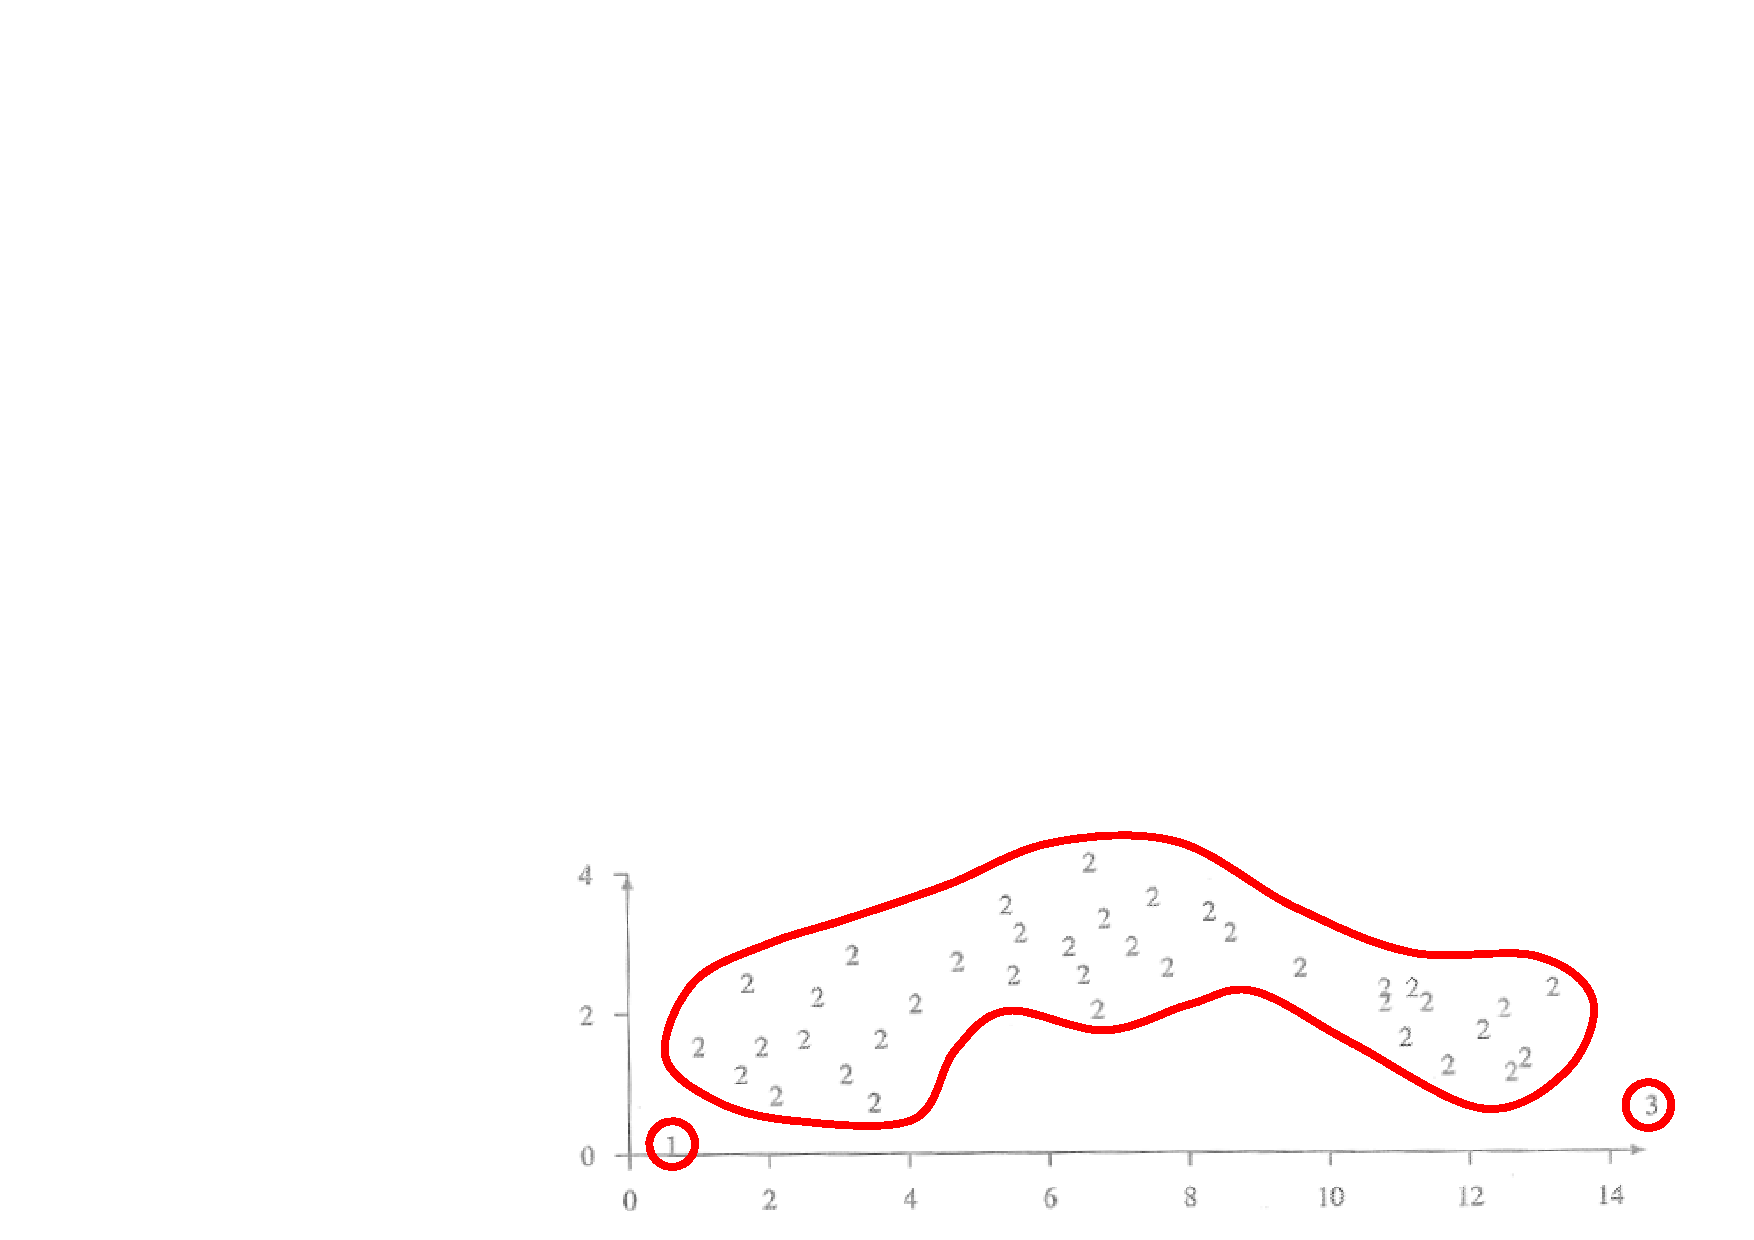
\includegraphics[angle=0,width=1\linewidth]{images/unsupervised/hierarchical/hierarchical_single_link_drawback_2.pdf}
%				\caption{Single-Link Dendogram Good K}
				%\label{Enel_QQ_Plot_Normal}
			\end{figure}

		\end{columns}


	%\end{block}

\end{frame}


\begin{frame}

	\frametitle{{\color{GradientDescentDiagramGreen}Hierarchical Clustering}: segmentazione}
	%\begin{block}{}

		\begin{figure}[!htbp]
			\centering
			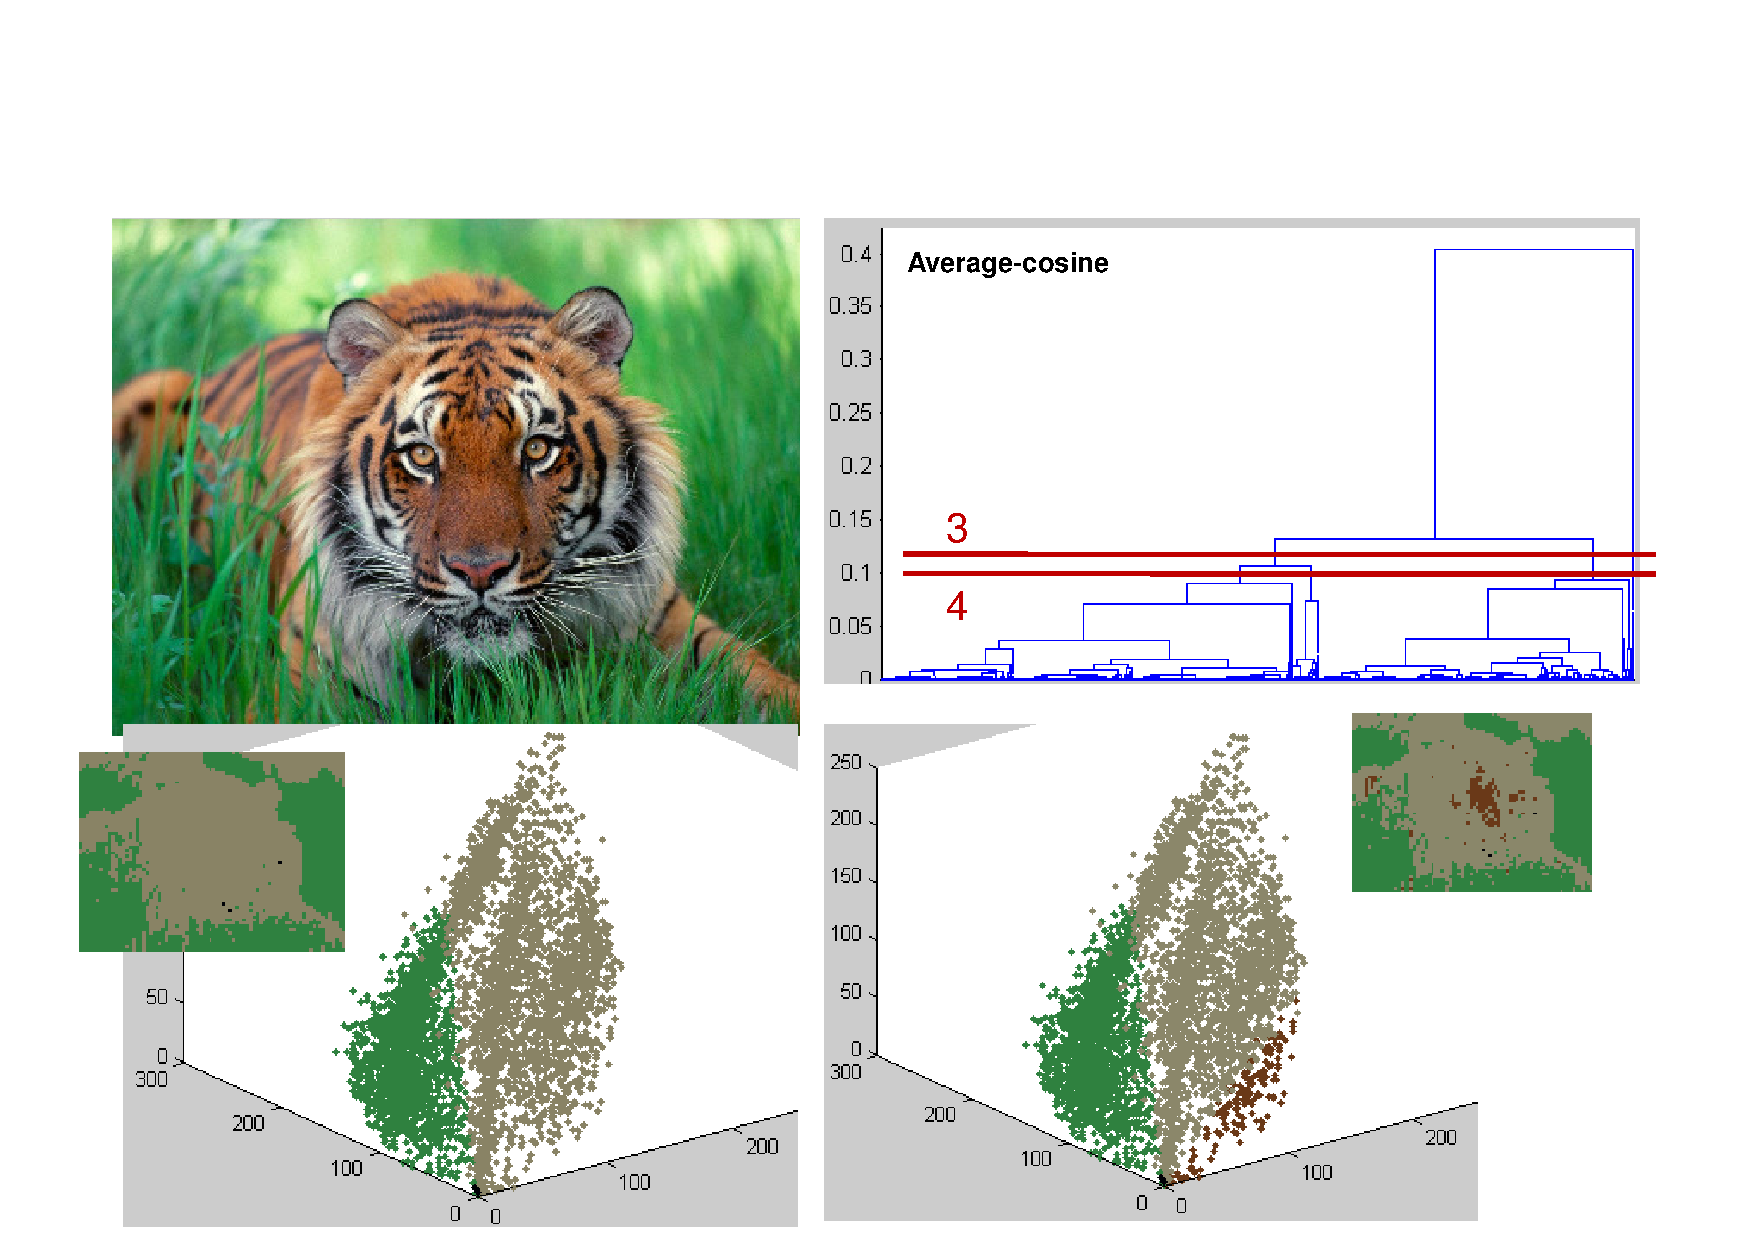
\includegraphics[width=11.0cm]{images/unsupervised/hierarchical/hc_avg_cosine_1.pdf}
			%\caption{Stripe Radar for Fraud Detection}
		\end{figure}

	%\end{block}

\end{frame}

\begin{frame}

	\frametitle{{\color{GradientDescentDiagramGreen}Hierarchical Clustering}: segmentazione}
	%\begin{block}{}

		\begin{figure}[!htbp]
			\centering
			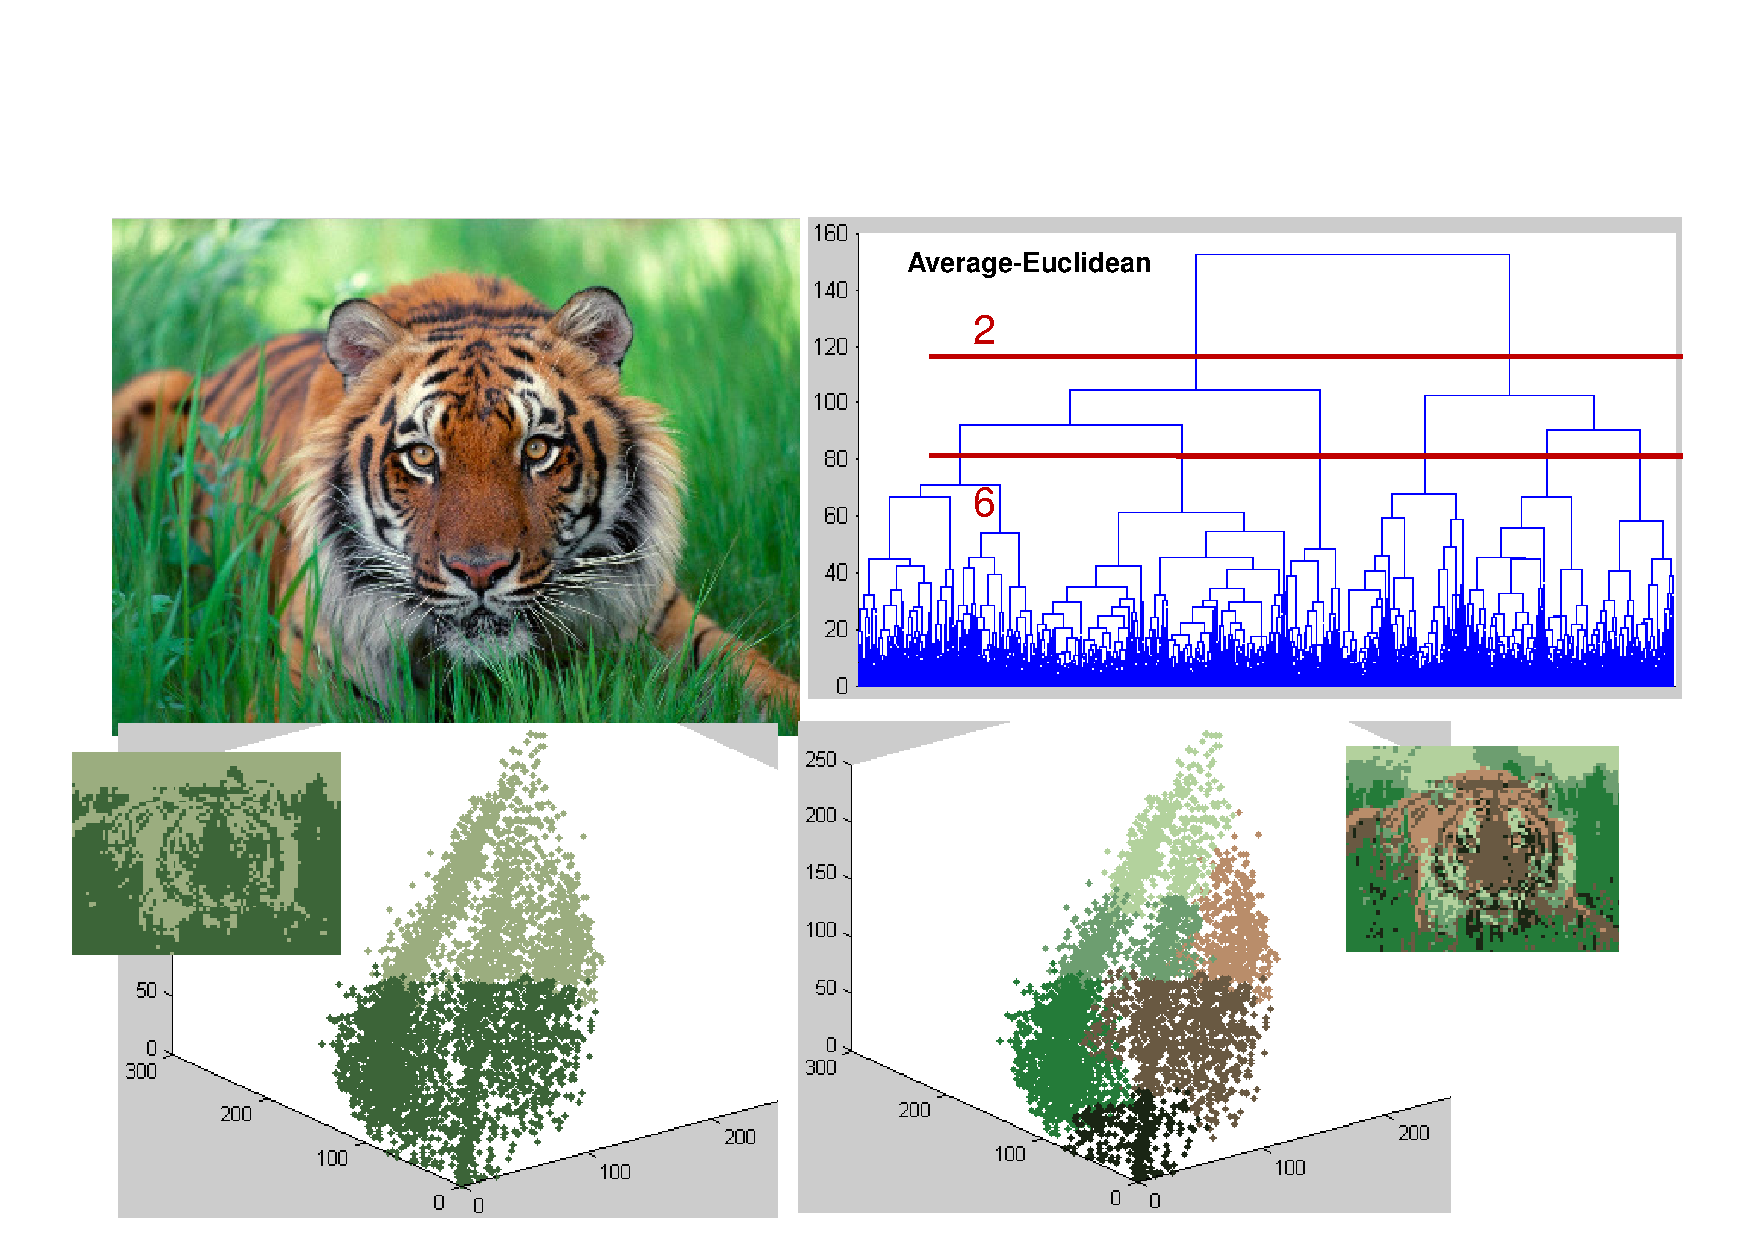
\includegraphics[width=11.0cm]{images/unsupervised/hierarchical/hc_avg_euclidean_1.pdf}
			%\caption{Stripe Radar for Fraud Detection}
		\end{figure}

	%\end{block}

\end{frame}


\begin{frame}

	\frametitle{{\color{GradientDescentDiagramGreen}Hierarchical Clustering}: segmentazione}
	%\begin{block}{}

		\begin{figure}[!htbp]
			\centering
			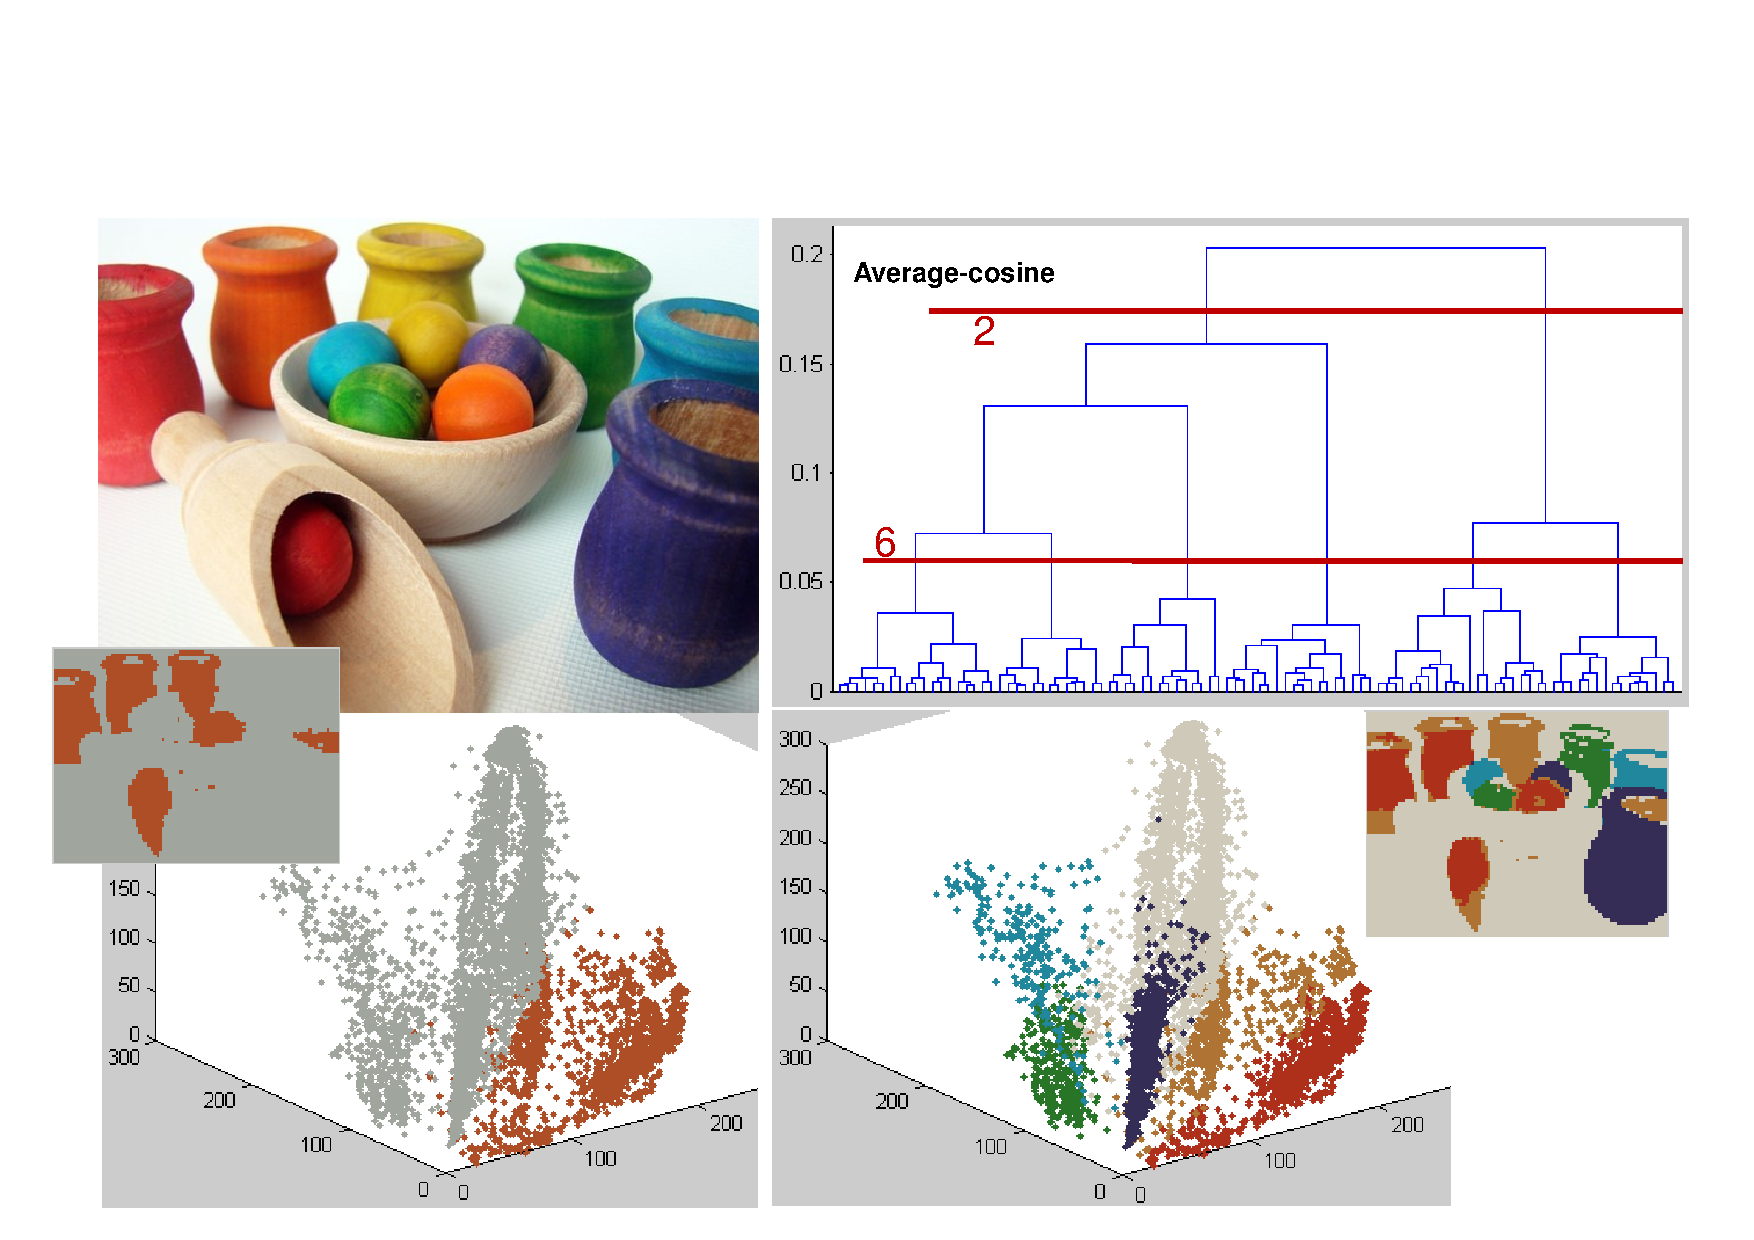
\includegraphics[width=11.0cm]{images/unsupervised/hierarchical/hc_avg_cosine_2.pdf}
			%\caption{Stripe Radar for Fraud Detection}
		\end{figure}

	%\end{block}

\end{frame}


\begin{frame}

	\frametitle{{\color{GradientDescentDiagramGreen}Hierarchical Clustering}: segmentazione}
	%\begin{block}{}

		\begin{figure}[!htbp]
			\centering
			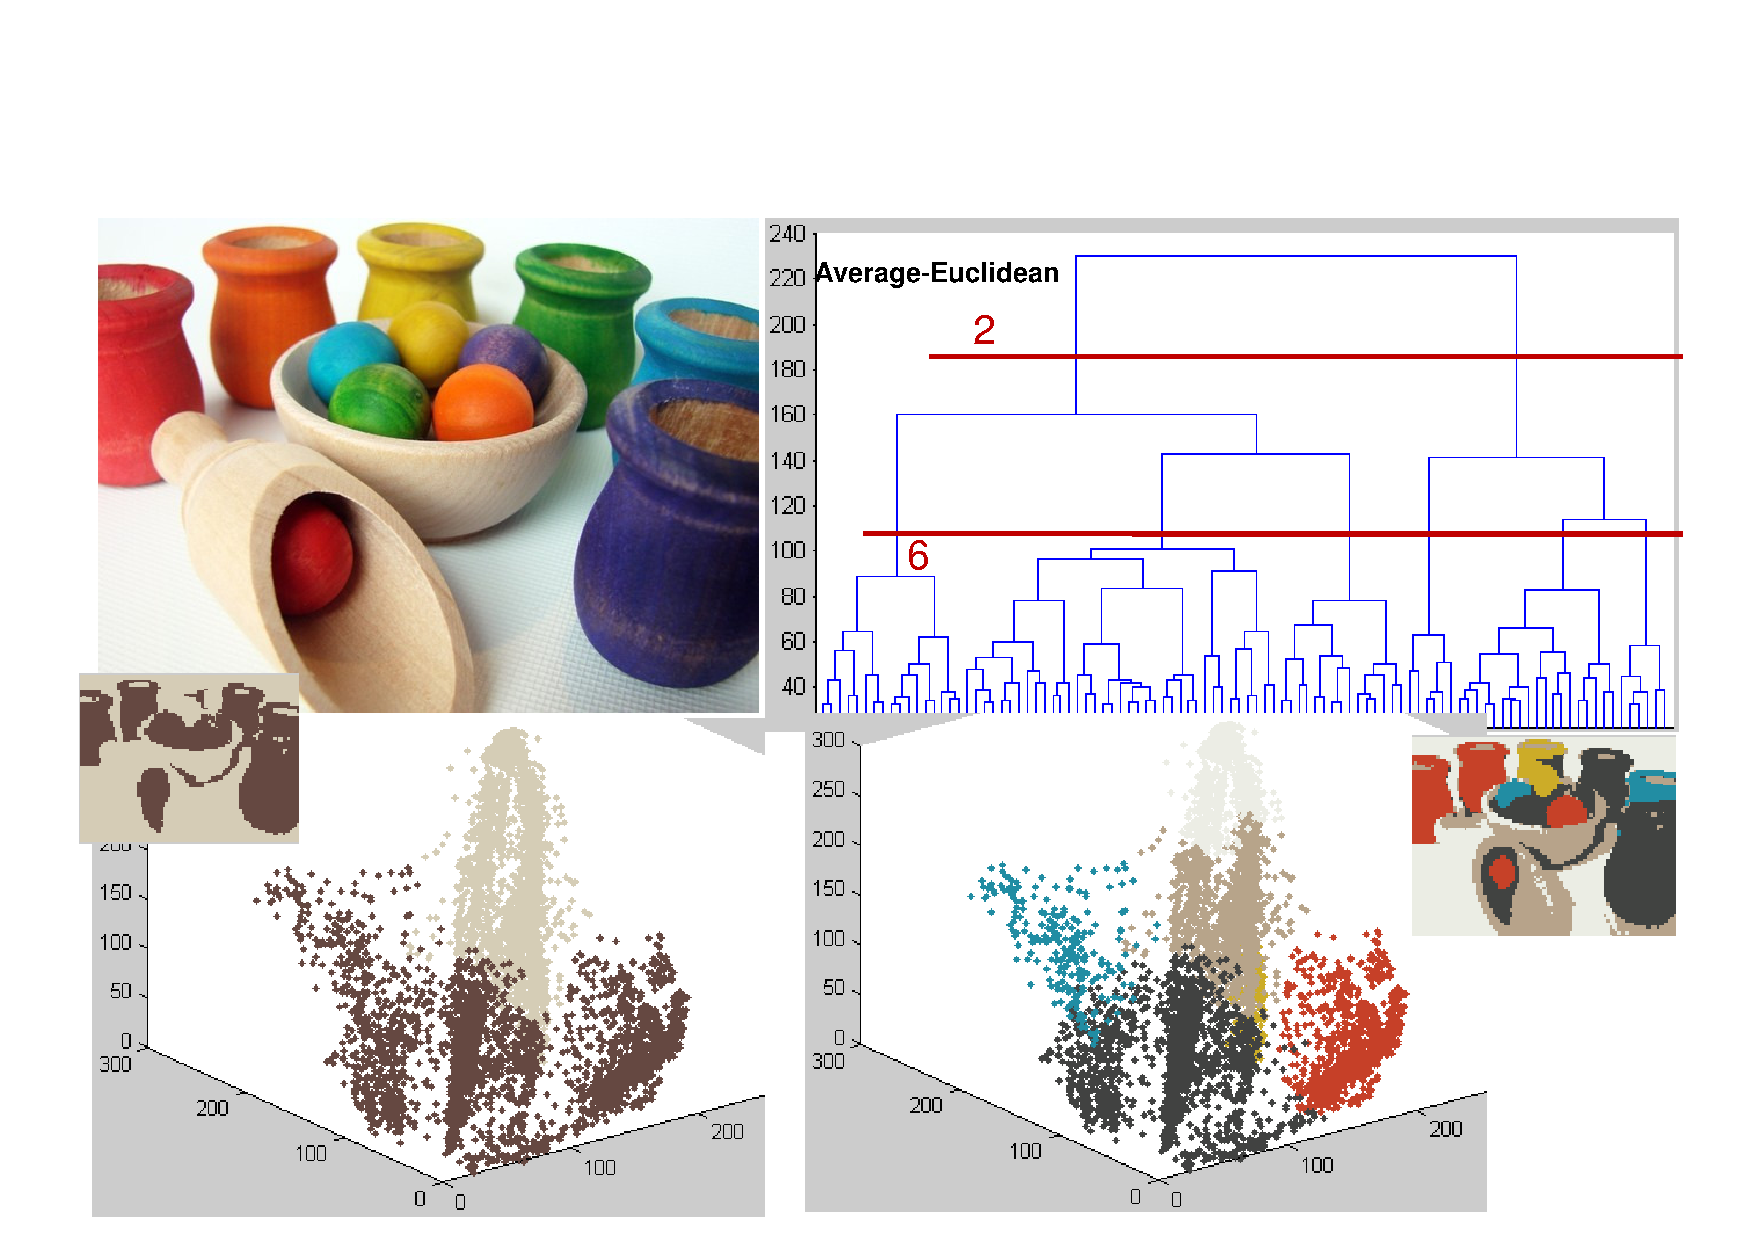
\includegraphics[width=11.0cm]{images/unsupervised/hierarchical/hc_avg_euclidean_2.pdf}
			%\caption{Stripe Radar for Fraud Detection}
		\end{figure}

	%\end{block}

\end{frame}


\begin{frame}

	\frametitle{{\color{GradientDescentDiagramGreen}Hierarchical Clustering}: pro e contro}
	%\begin{block}{}

		Pro e contro del clustering gerarchico:
		\begin{itemize}
			\item la procedura di clustering non richiede la definizione del numero di cluster
			\item la procedura di clustering produce relazioni gerarchiche tra i cluster
			\item non viene fornita un'identificazione esplicita del numero ottimale di clusters
			\item a seconda della strategia di linkage (in particolare single-link), sono possibili cluster eterogenei (chaining). In questi casi, rappresentare dei cluster con un unico punto è fuorviante
			\item gli algoritmi di clustering gerarchico agglomerativo o divisivo esaminano tutte le coppie di punti\ifthenelse{\boolean{highschool}}{}{ e hanno complessità rispettivamente di $O(n^2log(n))$ e $O(n^2)$}.
		\end{itemize}
	%\end{block}

\end{frame}
